\setAuthor{Richard Luhtaru}
\setRound{lahtine}
\setYear{2020}
\setNumber{G 4}
\setDifficulty{4}
\setTopic{TODO}

\prob{Noova}
\begin{wrapfigure}[12]{r}{0.15\linewidth}
		\vspace{10pt}
		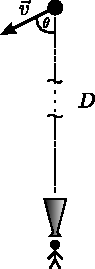
\includegraphics[width=1.1\linewidth]{2020-lahg-04-yl.pdf}
	\end{wrapfigure}
	Hobiastronoom Jarl vaatleb teleskoobiga noovaplahvatust ja mõõdab ühe plahvatuse ainejäänuki kiirust. On teada, et ainejäänuki tegelik kiirus on $v$ ja nurk kiirusvektori ja vaatesihi vahel on $\theta$.
	
	Jarl teab varasemate mõõtmiste põhjal, et noova kaugus on $D$, kuid ta ei tea nurka $\theta$. Seetõttu eeldab Jarl, et ainejäänuk liigub vaatesihiga risti ning arvutab kauguse ja jäänuki nurga muutumise abil jäänuki näiva kiiruse $v'$.
	
	Leia Jarli poolt mõõdetav näiv kiirus $v'$, eeldusel et noova on väga kaugel ($vt \ll D$, kus $t$ on vaatluse aeg) ning et kosmoloogiline paisumine on tühine. Valguse kiirus on $c$. Kas on võimalik, et ainejäänuki näiv kiirus $v'$ on mingi $v$ ja $\theta$ väärtuse korral valguse kiirusest suurem, isegi kui $v < c$?
	
	
	
\hint

\solu
Vaatleme jäänuki liikumist aja $t$ jooksul, selle aja jooksul liigub jäänuk vahemaa $vt$. Näeme, et ristisihis liigub jäänuk vahemaa $vt \sin \theta$, seega kasutades väikeste nurkade lähendusi, on Jarli poolt mõõdetav nurk nende kahe positsiooni vahel $\alpha = vt\sin\theta/D$ ja näiv vahemaa, mille jäänuk nende hetkede vahel läbib on
\begin{equation*}
	x' = \alpha D = vt\sin\theta.
\end{equation*}

\begin{figure}[h]
\centering
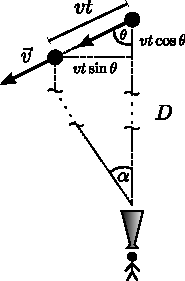
\includegraphics[width=0.25\linewidth]{2020-lahg-04-sol.pdf}
\end{figure}

Küll aga tuleb arvestada ka sellega, et jäänuk liigub selle aja jooksul $vt \cos\theta$ vaatesihis Jarlile lähemale, mistõttu teepikkus, mille valgus peab Jarlini jõudmiseks läbima, lüheneb ja seega näiv aeg kahe hetke vahel $t'$ ei ole võrdne tegeliku ajaga $t$. Kuna esimesel hetkel on jäänuki kaugus Jarlist $D$ ning teisel juhul $D-vt\cos\theta$ (kasutades lähendust, et $D$ on väga suur), siis näiv aeg kahe hetke vahel on
\begin{equation*}
t' = t_2 - t_1 = \left(t + \frac{D-vt\cos\theta}{c}\right) - \frac{D}{c} = t\left(1 - \frac{v\cos\theta}{c}\right).
\end{equation*}

Seetõttu Jarli poolt mõõdetav näiv kiirus on
\begin{equation*}
v' = \frac{x'}{t'} = \frac{v \sin \theta}{1- \frac{v}{c}\cos\theta}.
\end{equation*}

Näeme, et näiv kiirus võib olla tõesti suurem kui $c$. Näiteks kui $\theta = 45^\circ$ ja $v = \frac{7}{5\sqrt 2}c$ (mis on väiksem kui $c$), siis
\begin{equation*}
v' = \frac{\frac{7}{5\sqrt 2} c \cdot \frac{1}{\sqrt 2}}{1- \frac{7}{5\sqrt 2} \cdot \frac{1}{\sqrt 2}} = \frac{7}{3} c > c.
\end{equation*}

\textit{Märkus.} Selline nähtust, kus näiv kiirus on valguse kiirusest suurem (ingl. k. \textit{superluminal motion}), on märgatud mitmete astronoomiliste objektide korral. Üks suuremaid näivaid kiirusi on mõõdetud kvasarijoa korral, mille näivaks kiiruseks mõõdeti $\num{9.6}c$.
\probend